\documentclass[tesis.tex]{subfiles}

%\newcommand{\ol}{\overline{}}
%\newcommand{\ic}{independiente de contexto }
%\newcommand{\APND}{automáta de pila no determinístico }
%\newcommand{\APD}{automáta de pila determinístico }
%\newcommand{\fg}{grupo finitamente generado }
%\newcommand{\fp}{grupo finitamente presentado }
%\newcommand{\vl}{virtualmente libre}
%\newcommand{\WP}{\text{WP}(G, \Sigma)}
%\newcommand{\deriva}{\overset{*}{\Rightarrow_{\cal G}}}
%\newcommand{\cG}{ {\cal G} }



\begin{document}
	
\chapter{Grupos virtualmente libres.}
En este capítulo veremos como entran en juego las diferentes áreas de la matemática para definir de manera equivalente a los grupos virtualmente libres.

\begin{deff}
Un grupo $G$ finitamente generado es \blue{virtualmente libre} si existe un subgrupo libre $F$ tal que su índice en $G$ es finito.
\end{deff}

Veamos algunas propiedades elementales que cumplen todos los grupos \vl. 
Antes probemos algunos lemas sobre grupos.
\begin{deff}
	Sea $G$ un grupo y $H$ un subgrupo entonces el normalizador de $H$ en $G$ es el siguiente subgrupo
	\begin{equation*}
		N_G(H) = \{ g\in G : gHg^{-1} = H  \}
	\end{equation*}
\end{deff}

Denotaremos por $S= \{ g \in G :  gHg^{-1} \}$ al conjunto de conjugados del subgrupo $H$. 

\begin{lema}\label{lema_normalizador_conjugados}
	Si $G$ es un grupo \fg y $H$ es un subgrupo de índice finito entonces $N_G(H)$ tiene índice finito y más aún $[G:N_G(H)] = |S|$.
\end{lema}
\begin{proof}
	Para ver que tiene índice finito notemos que $H \le N_G(H)$ por lo tanto tenemos que 
	\[
		[G:N_G(H)] \le [G:H] < \infty.
	\]
	
	Para probar la otra afirmación definimos la siguiente función hacia los cosets a derecha del normalizador desde el conjunto $S$,
	\begin{align*}
		S  &\to  G/N_G(H) \\
		sHs^{-1} &\mapsto N_G(H)s
	\end{align*}
	Veamos que es biyectiva.
	
	Si $N_G(H)s = N_G(H)t$ entonces tenemos que esto sucede si y solo sí $st^{-1} \in N_G(H)$.
	Esto nos dice que por la definición del normalizador,
	\[
		st^{-1} H ts^{-1} = H \iff s^{-1}Hs = t^{-1}Ht
 	\]
 	y de esta manera obtenemos que la función está bien definida y es biyectiva.
\end{proof}

\begin{lema}\label{lema_indice_interseccion}
	Sea $G$ un grupo \fg \  y sean $K,H$ subgrupos de índice finito entonces $K \cap H$ es un subgrupo de índice finito.
\end{lema}
\begin{proof}
	Primero notemos que por el segundo teorema de isomorfismo para grupos tenemos que existe una biyección entre los siguientes conjuntos,
	\[
		KH / K \simeq K / K \cap H
	\]
	y en particular como $|KH / K| \le |G / K| < \infty$ por hipótesis obtenemos así que $|K / K \cap H| < \infty$.
	
	Finalmente por una propiedad de índices de subgrupos obtenemos lo siguiente
	\[
		[G:K\cap H] = [G:K][K: K \cap H]
	\]
	 y como ambos índices de la derecha son finitos por lo visto obtenemos que $K \cap H$ es un subgrupo de índice finito también tal como queríamos ver.
\end{proof}

\begin{lema}\label{lema_subg_fg}
	Sea $G$ un \fg y sea $H$ subgrupo de índice finito entonces $H$ es un \fg.
\end{lema}
\begin{proof}
	Sea $A = \{g_1, \dots, g_n\}$ conjunto finito de generadores de $G$.
	Sea $T =\{t_1, \dots, t_m\}$ conjunto transversal a derecha de $H$, esto es que $Ht_1, \dots, Ht_k$ son todos los cosets a derecha de $H$ sobre $G$.
	Supongamos que $t_1=1$ dado que es el representante del coset $H$.

	Dado $g_j$ generador de $G$ debe existir $h_{ij} \in H$ tal que $h_{ij}t_{k} = t_ig_j$ para cierto $t_k$.
	También debe existir $h_i \in H$ de manera que $ h_i t_{k} = g_i$ para cierto $t_k$.
	Veamos que el conjunto finito 
	\[
		B = \{ h_{ ij}  \}_{1 \le i,j \le n } \cup \{ h_i \}_{1 \le i \le n}
	\]
	 genera a $H$.
	
	Dado $h \in H$ tenemos que 
	\[
		h = g_{i_1}\dots g_{i_r}
	\]
	donde usamos el conjunto finito de generadores de $G$.
	
	Por lo visto anteriormente podemos escribir  $g_{i_1} = h_{i_1}t_{k_1}$ y entonces nos queda la siguiente escritura de $h$,
	\[
		h = h_{i_1}t_{k_1} g_{i_2}\dots g_{i_r}
	\]
	entonces usando que $h_{k_{1}i_{2}}t_{k_2} = t_{k_1}g_{i_2} $ llegamos a la siguiente escritura de $h$,
	\[
	h = h_{i_1}h_{k_{1}i_{2}}t_{k_2}\dots g_{i_r}.
	\]
	Repitiendo inductivamente este procedimiento llegamos a que $h =h_{i_1}h_{k_{1}i_{2}} \dots t_{k_r}$.
	Este $t_{k_r}$ tiene que ser $1$ porque justamente $h \in H$, por lo tanto tenemos $B$ es un conjunto finito de generadores de $H$.
\end{proof}


Con esto podemos probar estos resultados elementales de grupos \vl.

\begin{prop}\label{prop_vls}
	Para todo grupo $G$ \vl \ valen las siguientes propiedades.
	\begin{enumerate}
		\item Si $F$ es un subgrupo libre de índice finito entonces podemos tomarnos otro subgrupo $F'$ de manera que sea normal, libre y de índice finito.
		\item Si $H$ es un subgrupo de $G$ de índice finito entonces $H$ también resulta ser \vl.
	\end{enumerate}
\end{prop}

\begin{proof}
	\begin{enumerate}
		\item Si $G$ es virtualmente libre y $F$ es un subgrupo libre tenemos que la cantidad de conjugados de $F$ es finita por el lema \ref{lema_normalizador_conjugados}.
		Por lo tanto podemos considerar el siguiente subgrupo normal
		\[
		F' = \bigcap_{g \in G} gFg^{-1}
		\]
		donde la cantidad de grupos que estamos intersecando es finita y es normal por construcción.
		Veamos que $F'$ nos sirve. 
		Para ver que tiene índice finito nos alcanza con usar el lema \ref{lema_indice_interseccion} e inducción para que valga para una intersección finita arbitraria.
		Como tiene índice finito usando \ref{lema_subg_fg} sabemos entonces que es un \fg.
		Finalmente notemos que es libre por el resultado \ref{coro_niels_sch} que nos dice que todo subgrupo de un grupo libre es libre, en particular al ser $F'$ subgrupo de $F$ que es libre obtenemos que $F'$ es libre tal como queríamos ver.
		
		\item Por el lema \ref{lema_subg_fg} obtenemos directamente que $H$ es \fg.
		Si $F$ es un libre de índice finito en $G$ podemos tomar $H \cap F$ que es libre por ser subgrupo de un libre de acuerdo al resultado \ref{coro_niels_sch}.
		El índice resulta ser finito puesto que 
		\[
			[H:F\cap H] \le [G:F] < \infty.
		\]
	\end{enumerate}
\end{proof}

\begin{obs}\label{obs_presentacion_vl}
	Dado $G$ \vl \ vamos a construirnos una presentación en particular.
	
	Como es un grupo \vl \ tenemos $F$ subgrupo libre que podemos tomarlo normal y $G/F$ grupo finito de manera que podemos escribir a $G$ como una extensión de estos dos grupos por medio de la siguiente forma
	\begin{center}
		\begin{tikzcd}
			1 \arrow[r] & F \arrow[r, "\iota"] & G \arrow[r, "\pi"] & G/F \arrow[r] & 1
		\end{tikzcd}
	\end{center}
	
	Consideremos que $F$ es libre generado por $Y = \{ y_1, \dots, y_n \}$.
	Por otro lado sea $G/F = \{ b_i : 1 \le i \le m \}$ todos los elementos de este conjunto finito.
	Elegimos un transversal a derecha $T = \{ t_1, \dots, t_m \}$ de manera que $\pi(t_i)= b_i$ y $t_1 = 1$.
	
	Dado que es un transversal tenemos que se deben cumplir las siguientes dos relaciones para $y_j \in Y$ y $t_i,t_j,t_k \in T$. 
	\begin{enumerate}
		\item $t_iy_jt_i^{-1} = u_{ij}$ donde $u_{ij} \in F$ usando que $F$ es normal.
		\item Si tenemos que $b_ib_j = b_k$ entonces $t_it_j = z_{ij}t_k$ donde $z_{ij} \in F$ usando que $(Ht_i)(Ht_j) = Ht_k$.
	\end{enumerate}
	
	Afirmamos que la siguiente es una presentación finita de $G$.
	\[
		\langle W \mid R \rangle =  \langle y_1, \dots, y_n, t_1, \dots, t_m \mid t_iy_jt_i^{-1} = u_{ij},  t_it_j = z_{ij}t_k \rangle.
	\]
	Sea el grupo que genera este presentación $H$ y sea $F'$ el grupo libre sobre sus generadores.
	
	Notemos que $W =Y \cup T$ genera a $G$ porque justamente $F$ es libre y generado por $Y$ y $T$ es un conjunto transversal finito porque $F$ tiene índice finito en $G$.
	Esto nos dice que tenemos un epimorfismo de grupos de $F'$ en el grupo $G$.
	
	Toda relación de $G'$ la cumple el grupo $G$ por la elección que tomamos, de esta manera tenemos un epimorfismo de grupos $\ol \varphi$ tal que hace conmutar al siguiente diagrama,
	
	\begin{center}
		\begin{tikzcd}
			F' \arrow[dd] \arrow[rr, "\varphi"]          &  & G \\
			&  &   \\
			H \arrow[rruu, "\overline \varphi"', dashed] &  &  
		\end{tikzcd}
	\end{center}
	
	El grupo  $G$ es tal que a toda palabra $w$ en sus generadores la podemos llevar a que sea de la pinta
	\[
		w = yt
	\]
	donde $y \in F$ reducida y $t \in T$ es alguno de los transversales. 
	Para llegar a esto hacemos el mismo procedimiento que hicimos en la demostración del lema \ref{lema_subg_fg}.
	
	De esta manera una palabra es trivial si y solamente si $y=1$ y $t=1$. 
	Esto nos dice que $\ol \varphi(w) = 1$ si y solamente si $w=1$. 
	Concluimos así que $\ol \varphi$ es un isomorfismo de grupos tal como queríamos ver y por lo tanto  $\langle W \mid R \rangle$ resultó ser una presentación de $G$.
	
\end{obs}
\medskip

Veamos ahora unos ejemplos y contrajemplos de grupos \vl s.

\begin{ej}
Veamos algunos ejemplos elementales de grupos que son de esta familia y algunos que no lo sean.
\begin{enumerate}	
	\item Cualquier extensión de un grupo libre por un grupo finito es un grupo virtualmente libre,
	\[
		1 \to F \to G \to K \to 1
	\]
	donde $K$ es un grupo finito y $F$ es un grupo \fg libre.
	En particular esto nos da los casos más elementales de productos directos y semidirectos, esto es $G= F \times K$ o bien  $G = F \ltimes K$.
	En este capítulo veremos que todo grupo \vl \ podemos considerarlo como un subgrupo de una extensión de este tipo.
	
	\item El ejemplo más sencillo de un grupo que no es \vl \ es $\ZZ \times \ZZ$.
	La primera observación es que al ser abeliano si tiene un subgrupo libre necesariamente tiene que ser isomorfo a $\ZZ$.
	
	Nos alcanza con ver que no es virtualmente $\ZZ$.
	Sea $F$ un subgrupo que es isomorfo a $\ZZ$.
	Sea $(n,m) \in \ZZ \times \ZZ$ el generador de $F$.
	Probaremos que $\ZZ \times \ZZ / F$ tiene orden infinito.
	Para eso consideraremos $(p,q) \in \ZZ \times \ZZ$	tal que $p,q$ son primos distintos y ambos coprimos con $m,n$.
	Veamos que $[(p,q)] \in \ZZ \times \ZZ / F$ tiene orden infinito.
	Si no lo fuera deberían existir $\alpha, \beta \in \ZZ$ de manera que 
	\begin{align*}
		\alpha (p,q) = \beta(n,m) 
	\end{align*}
	
	como todos son coprimos entre sí esto nos dice que $p \mid \beta$ y similarmente que $q \mid \beta$, por lo que tenemos que $q \mid \alpha$ y $p \mid \alpha$.
	Esto nos dice que se pueden escribir de esta manera
	\begin{align*}
		\alpha = p^{r_1} q^{s_1} \gamma_1 \\
		\beta = p^{r_2} q^{s_2} \gamma_2
	\end{align*}
	con $r_i, s_i \ge 1$ para $i=1,2$.

	Finalmente como 
	\[ 
		\alpha p = \beta n
	\]
	tenemos que $r_1+ 1 = r_2$ pero por otro lado como
	\[
		\alpha q  = \beta m
	\]
	acá tenemos que al ser $m$ coprimo con $p$ luego la multiplicidad de $p$ en la descomposición en primos de lo que está a la izquierda es $r_2 - 1 $ mientras que lo que está a la derecha es $r_2$.
	
	Esto es una contradicción que vino de suponer que $[(p,q)] \in \ZZ \times \ZZ / F$ tenía orden finito por lo tanto tenemos que $\ZZ \times \ZZ$ no puede ser \vl.
	
\end{enumerate}
\end{ej}






\section{Grupos independientes de contexto.}
% 
%\begin{deff}
%	Si $G$ es un grupo \fg tal que para ciertos generadores $\Sigma$ resulta que $WP(G, \Sigma)$ es independiente de contexto entonces diremos que $G$ es un \blue{grupo \ic }.
%\end{deff}

%
%\begin{ej} Consideremos los siguientes ejemplos.	
%	\begin{enumerate}[E1.]
%		\item 
%		Dado $F$ grupo libre de rango finito supongamos generado por el conjunto finito $X$. 
%		Sea  $Y = X \cup X^{-1}$ el conjunto de generadores simétrico de $X$. 
%		Probemos que $\text{WP}(F,Y)$ es un lenguaje independiente de contexto.
%		
%		Consideremos el siguiente autómata de pila,
%		\[
%			M = (\{ 1 \}, Y, Y, \delta, 1, \{1\}).
%		\]
%		
%		Por como lo definimos tiene un solo estado y el alfabeto tanto de entrada como el de la pila que usa es el conjunto de generadores $Y$.
%		La función de transición $\delta$ está definida de la siguiente manera,
%		\[
%		\delta(1, y_i, u)=\left\{
%		\begin{array}{ll}
%			(1 , u )  &\ \text{si} \ a = 1  \\
%			(1, y_i \cdot u') &\ \text{si} \  u = y_jw'  \\
%		\end{array}
%		\right.
%		\]
%		donde al apilar hacemos la multiplicación $y_i \cdot u$ en el grupo libre $F$.
%		
%		Consideremos el lenguaje aceptado por pila vacía, esto es
%		
%		\[
%		{\cal L }(M) = \{  y \in Y^* \mid (y,1,1)   \vdash^*  (1, 1, 1)  \}.
%		\]
%		
%		Notemos que ${\cal L }(M) = \text{WP}(F,Y)$ porque justamente en la pila apilamos lo que vamos leyendo de izquierda a derecha y desapilamos cuando leemos el inverso del generador que está en el tope de la pila.
%		Esto es que desapilamos cuando un generador aparece después de su inverso en la palabra.
%	
		
%		Dado un grupo libre $F$ veamos cómo construir un automáta $\cal M$ tal que acepta su problema de la palabra. 
%		
%		Pensemos un \APND que tenga dos estados. Uno inicial que también va a ser final para poder aceptar la palabra vacía que corresponde al elemento 1 de nuestro grupo y otro estado para las palabras que no están en el problema de la palabra.
%		Para eso la idea es tener en la pila lo que fuimos leyendo de nuestra palabra hasta el momento visto como un elemento en el grupo. 
%		Esto es, cada vez que leemos una letra de la palabra ver de multiplicarla como un elemento en el grupo con lo que tenemos en el tope de la pila. 
%		Eventualmente cuando hayamos recorrido la palabra entera debería quedarnos una palabra en la pila que queremos que sea exactamente $1$ y esto es lo mismo que pedir que sea aceptada por pila vacía. 
%		Entonces este automáta lo podemos representar de la siguiente manera:	
%		
%		\begin{center}
%			\begin{tikzpicture}[->,>=stealth',shorten >=1pt,auto,node distance=4.5cm,
%				scale = 1.15,transform shape]
%				
%				\node[state,accepting,initial] (1') {$1'$};
%				\node[state] (1) [right of=1'] {$1$};
%				
%				\path (1') edge[bend left]              node {} (1)
%				(1) edge[bend left]              node {} (1');
%			\end{tikzpicture}
%		\end{center}
%		
%		
%		Donde las transiciones del estado 1' a 1 son todas las transiciones en las cuales la letra que estamos por leer no es la inversa de lo que esté al tope de la pila. Por otro lado las transiciones del estado 1 al estado 1' son todas las que lo que leemos es justamente el inverso de lo que está al tope de la pila.
		
%		\item 	$\ZZ \times \ZZ$ no es un grupo independiente de contexto.
%		Si tomamos los siguientes generadores como monoide $\Sigma = \{ a,b,c \}$ tal que tenemos un morfismo de monoides $\pi: \Sigma^* \to \ZZ \times \ZZ$ dado por $\pi(a)=(1,0), \pi(b)=(0,1), \pi(c)=(-1,-1)$.
%		Bajo esta presentación 
%		\[
%		WP(\ZZ \times \ZZ, \Sigma) = \{ w \in \Sigma^*  : \ \exists n \in \NN, \ |w|_a = |w|_b = |w|_c = n \}.
%		\]
%		Este lenguaje no es independiente de contexto.
%		Para eso usemos el lema del pumping \ref{pumping} para probarlo por contradicción.
%		Si fuera \ic debería existir una constante $n \ge 0$ tal que hace valer las hipotesis del lema.
%		Consideremos la palabra $w = a^n b^n c^n \in WP(G, \Sigma)$.
%		Si tenemos una factorización 
%		\[
%		uvwxy = a^nb^nc^n
%		\]
%		 si $|vwx| \le n$ implica que no todas las letras aparecen en $vwx$.
%		Supongamos que la letra que no aparece es $c$.
%		Por otro lado como $|vx| \le 0$ esto nos dice que al menos una letra aparece en la subpalabra $vx$.
%		Si tomamos $i=0$ notemos que la palabra $uwy \in WP(G,\Sigma)$ pero esto es una contradicción porque la cantidad de $c$ en esta palabra es mayor que de $a$ o $b$.
%		
%	\end{enumerate}
%	
%\end{ej}

\begin{obs}\label{palabras-wp}
	Si tenemos un grupo $G$ tal que es independiente de contexto consideremos $\cal G$ gramática que genera al lenguaje del problema de la palabra, $\WP = L(\cal G)$.
	Si $A$ es una de las variables de esta gramática podemos obtener el lenguaje $L_A$ de palabras generadas a partir de esta variable, donde
	\[
	L_A = \{ w \in \Sigma^*  \ | \ A \deriva w  \}.
	\]
	Veamos que si $v,v' \in L_A$ entonces $v =_G v'$, es decir son el mismo elemento vistos en el grupo $G$. 
	Para eso si tenemos una derivación que en algún momento llega a $S \deriva \beta A \gamma \deriva uvw$ también tenemos otra derivación que deriva en $S \deriva \beta A \gamma  \deriva uv'w$. 
	Es decir que $uvw, u'v'w' \in \WP$ por lo tanto 
	\begin{equation*}
		uvw =_G 1 =_G uv'w \implies v =_G v'
	\end{equation*}
	tal como queríamos ver.
\end{obs}



Una pregunta natural es intentar entender la relación entre la clasificación del lenguaje del problema de la palabra de un grupo dado y las distintas familias de grupos que le corresponden. 
La siguiente demostración generaliza la construcción del ejemplo del problema de la palabra de un grupo libre.


\begin{teo}\cite{muller1983groups}
	Todo grupo virtualmente libre es independiente de contexto.
\end{teo}

 
\begin{proof}
	Sea $G$ grupo \vl  \ y consideremos una presentación $\langle W  \mid  R \rangle$ como la que construimos en la observación \ref{obs_presentacion_vl}.
	Veamos de construir un autómata de pila de manera que acepte al lenguaje $\text{WP}(G,W)$.
	Antes de definirlo consideremos algunos conjuntos finitos que nos van a servir para definir al autómata.
	
	Si tenemos que $ t_j y_i = u_{ij} t_j $ y que $ t_it_j = z_{ijk}t_k $ luego consideremos la siguiente definición.
	El conjunto finito $U = \{ u_{ij}, \ z_{ijk} : 1 \le i,j,k \le n \}$.
	Consideremos $\text{Pre}(U) = \{ u' \in Y^* : u'v \in U  \}$ el conjunto de los prefijos de las palabras en $U$ que sabemos es finito también.	
	Sea entonces el conjunto finito $Q = T \times T \cup Y \times \text{Pre}(U) $.
		
	Con estas definiciones ahora nuestro autómata lo definimos así: 
	\[
	{\cal M }= (Q, W , Y, \delta, (1,1,1), \{(1,1,1)\})
	\]
	El conjunto $Q$ van a ser nuestros estados.
	El alfabeto de entrada es $W$ que es el conjunto de generadores del grupo.
	El alfabeto de la pila es $Y$ que es el conjunto de generadores del subgrupo libre $F$.
	Nuestro estado inicial que también es el final corresponde a $(1,1,1)$.
		
	Ahora podemos definir la función de transición. 
	Sea $w_i \in W$ algún generador del grupo luego tenemos que
	\begin{align*}
		\delta(y_iw',(t_j,1,1), v) &= (w', (t_j,y_i,1), v) \\
		\delta(t_iw',(t_j,1,1), v) &= (w', (t_k,t_i,1), v) \\
	\end{align*}
	de manera que si estamos en $T \times \{ 1 \} \times \{ 1 \}$ podemos pasar a la segunda coordenada correspondiente a la letra de $W$ que hayamos leído.	
	Ahora en esta instancia lo que vamos a hacer es la reducción del producto de $u_{ij} \cdot v$ o bien el de $z_{ijk} \cdot v$ respectivamente una letra a la vez.
	Para esto tenemos
	\begin{equation*}
		\delta(w',(t_j,w_i,u), v) = (w', (t_j,w_i,y_iu), y_i \cdot v) .
	\end{equation*}
	siempre y cuando $y_iu$ sea un prefijo de la palabra de $U$ correspondiente.
	Notemos que sigue siendo determinístico porque fijamos de antemano alguna escritura única en los generadores $Y$ para cada palabra $u \in U$.
	En la pila hacemos la reducción en el grupo libre de multiplicar por una letra.
	Finalmente la función de transición la definimos para que podamos volver una vez que ya reducimos toda la palabra $u \in U$.
	Para eso tenemos 
	\begin{equation*}
		\delta(w',(t_j,w_i,u), v) = (w', (t_j,1,1), v).		
	\end{equation*}
	en el caso que $u \in U$, es decir que ya hicimos toda la reducción.
	
	Una vez definido este autómata consideremos ahora el lenguaje aceptado por pila vacía y estado final a la vez,
	
	\[
		{\cal L }(M) = \{  w \in W^* \mid (w,1,1)   \vdash^*  (1, 1, 1)  \}
	\]
	Debemos ver que el autómata acepta justamente al lenguaje que queremos. 
	Esto es que $ {\cal L }(M) = \text{WP}(G,W) $ 
	
	
	Dada una palabra $w \in W^*$ por como es esta presentación sabemos que se puede escribir como $w = vt$ donde $v \in F$ reducida y $t \in  T$. 
	De esta manera $w \in \text{WP}(G,W)$ si y solo si $v=1, t=1$.
	Notemos que el autómata en toda transición no hace más que reescribir la cadena de izquierda a derecha tal como hicimos en la observación \ref{obs_presentacion_vl}.
	Esto es que cuando termina de consumir la cadena de entrada llegamos a la configuración $(1, t_i, v)$ es decir que $w = vt_i$.
	Por lo tanto como aceptamos por estado final y pila vacía esto nos dice que $w \in \text{WP}(G,W)$ si y solo sí $w \in {\cal L}(M)$.
		
	Con esto probamos que los grupos virtualmente libres son \ic usando la equivalencia \ref{teo_ic_apnd}.
	
\end{proof}


El siguiente resultado es un teorema de Muller--Schupp demostrado en \cite{muller1985theory}.
La demostración sigue la exposición del paper \cite{diekert_contextfree_2017}.

\begin{teo} \cite{muller1985theory}
	Todo grupo independiente de contexto es tal que su grafo de Cayley tiene treewidth finito.
\end{teo}
\begin{proof}
La descomposición que hicimos en \ref{desc-grafo-cayley} es válida para todo grafo de Cayley. 
Veamos que esta descomposición para un grupo independiente de contexto tiene treewidth finito. 
Buscamos $k \in \NN$ tal que nos permita acotar $|\beta C| \le k$ para todo $\beta C \in V(T)$. 
Alcanza con ver que los diámetros de los bolsones $\beta C$ están acotados uniformemente, esto es que exista $M \in \NN$ tal que 
\[
\text{diam}(\beta C) =  \sup_{g,h \in \beta C} d(g,h) \le M
\] 
para todo $\beta C$ de la descomposición de árboles.
Si esto sucede, al ser el grupo finitamente generado por $\Sigma$ entonces $|\beta C| \le |\Sigma|^{M} < \infty$.


Dado que $G$ es un grupo independiente de contexto entonces el lenguaje del problema de la palabra para estos generadores $\WP$ tiene una gramática $\cal G$ independiente de contexto que lo genera. 
Consideremos que está en la forma normal de Chomsky.

Para cada variable $A$ de nuestra gramática podemos considerar el siguiente lenguaje
\[
L_A = \{ w \in \Sigma^* : A \deriva w  \}.
\]
Para este lenguaje introduzcamos un número natural $k_A \in \NN$ definido por $k_A = \min_{w \in L_A} |w|$. 
Como tenemos finitas variables en nuestra gramática $\cal G$ podemos considerar $k = \max_{A \in V} k_A$. 
Veamos que $\text{diam}(\beta C) \le 3k$ para todo $\beta C \in V(T)$.

Sean $g,h \in \beta C$ para cierta $C$ componente conexa de $V_n$, acotemos $d(g,h)$. 
Para eso consideremos una geodésica $\alpha$ que una $1$ con $g$ y análogamente otra $\gamma$ que una $1$ con $h$. 
Como $C \cup \beta C$ es conexo podemos tomar un arco $\tau$ que una $g$ con  $h$ dentro de $C \cup \beta C$. 
De esta manera tenemos un triángulo tal que si leemos las letras que están en la etiqueta del arco empezando desde $1$ y moviéndonos por $\alpha$ leemos la etiqueta $u$. 
Cuando nos movemos por $\tau$ leemos la etiqueta $v$. Consideremos que esta etiqueta $v$ es tal que $|v|>1$ caso contrario ya tenemos la cota probada. Finalmente leemos la etiqueta $w$ cuando regresamos al $1$ por medio de $\gamma$.
Como $uvw$ está en un ciclo en el grafo de Cayley entonces $uvw \in  \WP$ y por lo tanto tenemos alguna derivación $S \deriva uvw$.

Ya que tenemos esta derivación $S \deriva uvw$ miremos la primer variable que deriva a $v$ como subpalabra. 
Esto es que para la subpalabra $v$ sabemos que existe alguna variable $A$ tal que $A \deriva v'v''$ donde $v$ es a su vez una subpalabra de $v'v''$. 
Tomamos la última variable que aparece en la derivación.
%Esto es que para la subpalabra $v$ sabemos que debe existir alguna variable $A$ tal que $A \deriva u''vw''$ para $u''$ algún posfijo de $u$ y $w''$ algún prefijo de $w$ y aparece último en esta derivación. 
Ésta debe existir porque en particular $S$ cumple lo pedido de ser una variable que deriva a una palabra que contiene a $v$ como subpalabra.

Como está en la forma normal de Chomsky sabemos que al ser $|v| \ge 2$ entonces tenemos que la derivación tiene la siguiente pinta
\begin{equation*}
	S \deriva u'Aw' \Rightarrow_{\cal G} u'BC w' \deriva u'v'v''w'
\end{equation*}
donde $B,C$ son otras variables. En particular notemos que $A \deriva v'v''$, $B \deriva v'$ y $C \deriva v''$.


Si miramos la geodésica $\alpha$ sabemos que cuando leímos $u'$ habremos llegado a un vértice del grafo $x$, y al estar sobre la geodésica misma tenemos la siguiente igualdad,
%y que si tomamos el camino que leemos la palabra de menor longitud tenemos que habremos llegado al vértice $y$ que corresponde al haber leído $u'v'$.
\begin{equation*}
d(x,g) = d(1,g) - d(1,x).
\end{equation*}
Análogamente cuando miramos la geodésica $\gamma$ en la instancia que ya leímos $w'$ saliendo desde $h$ llegamos a cierto vértice $z$ y por la misma razón que en el caso anterior obtenemos
\begin{equation*}
	d(z,h) = d(1,h) - d(1,z).
\end{equation*}
Por otro lado si consideramos el vértice $y$ al que llegamos después de leer $u'v'$ que sabemos que está en el arco $\tau$ dado que $v$ es subpalabra de $v'v''$.
Usando que $y \in \tau \subseteq C \cup \beta C$ tenemos que $d(1,y) \le n+1 = d(1,g)$ por ser $C$ una componente conexa de $V_n$, entonces vale la siguiente desigualdad
\begin{equation*}
d(x,g) = d(1,g) - d(1,x) \le d(1,y) - d(1,x) = d(x,y)
\end{equation*}
y análogamente tenemos que $d(z,h) \le d(z,y)$.


Por la observación \ref{palabras-wp} notemos que si reemplazamos $v'$ por la palabra de menor tamaño del lenguaje $L_B$ seguimos teniendo un ciclo pero de longitud idéntica o más chica. 
La palabra $v'$ la leemos justamente cuando vamos del vértice $x$ al vértice $y$, así la distancia  $d(x,y)$ está acotada por la mayor de todas las palabras que puedan derivarse de $B$. 
Idénticamente hacemos esto para las variables $A$ y $C$.
Por como definimos a $k$ tenemos las siguientes cotas $d(x,y), d(y,z), d(x,z) \le k$.
%agregar dibujito, creo que es la manera más clara de explicar esto

\begin{figure}[H]
	\centering
	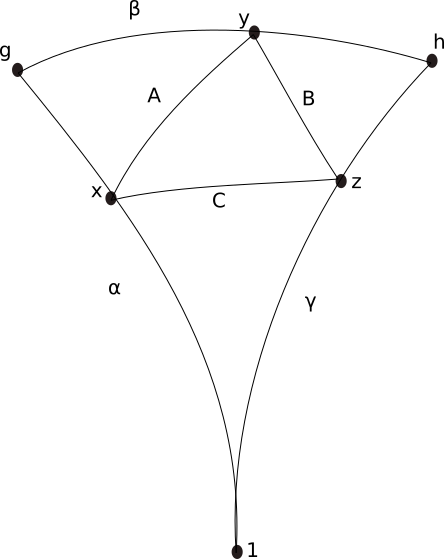
\includegraphics[scale=0.5]{treewidth.png}
	\caption*{}
\end{figure}



Ahora estamos listos para ver que $d(g,h) \le 3k$. Usamos la desigualdad triangular tres veces,
\begin{align*}
	d(g,h) & \le d(g,x) + d(x,z) + d(h,z) \\
	& \le d(x,y) + d(x,z) + d(y,z) \le 3k
\end{align*}
tal como queríamos ver.
\end{proof}

\begin{ej}
	Ejemplo de $PSL(2,\ZZ)$ o de algún otro grupo que sea un producto libre de grupos finitos.
\end{ej}






\end{document}